\documentclass{beamer}
\usepackage{tikz}
\usetikzlibrary{math}

\usepackage{pgfplots}
\usepgfplotslibrary{polar}

%Please read on the commands and options used below (either in the TikZ / PGFPlots manuals, or elsewhere).

\usepackage{filecontents}
% We're defining a file that will be created upon LaTeX compilation.
% Please note that you need to manually delete the file if you make changes,
% as filecontents does not overwrite files (for obvious security reasons).
\begin{filecontents*}{mpg.csv}
mpg,cylinders,displacement,horsepower,weight,acceleration,model_year,origin,name
18,8,307,130,3504,12,70,1,chevrolet chevelle malibu
15,8,350,165,3693,11.5,70,1,buick skylark 320
18,8,318,150,3436,11,70,1,plymouth satellite
16,8,304,150,3433,12,70,1,amc rebel sst
17,8,302,140,3449,10.5,70,1,ford torino
15,8,429,198,4341,10,70,1,ford galaxie 500
14,8,454,220,4354,9,70,1,chevrolet impala
14,8,440,215,4312,8.5,70,1,plymouth fury iii
14,8,455,225,4425,10,70,1,pontiac catalina
15,8,390,190,3850,8.5,70,1,amc ambassador dpl
15,8,383,170,3563,10,70,1,dodge challenger se
\end{filecontents*}

\begin{document}

\begin{frame}
  \begin{figure}
    \center
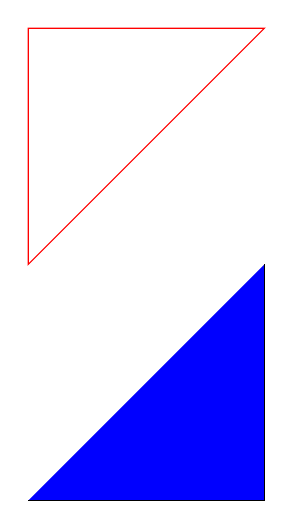
\begin{tikzpicture}[scale=3]
  \draw [fill=blue] (0, 0) -- (1, 0) -- (1, 1);
  \draw [red] (1, 2) -- (0, 2) -- (0, 1) -- cycle;
\end{tikzpicture}
    \caption{Example 1: Vector drawing in TikZ}
  \end{figure}
\end{frame}

\begin{frame}
  \begin{figure}
    \centering
    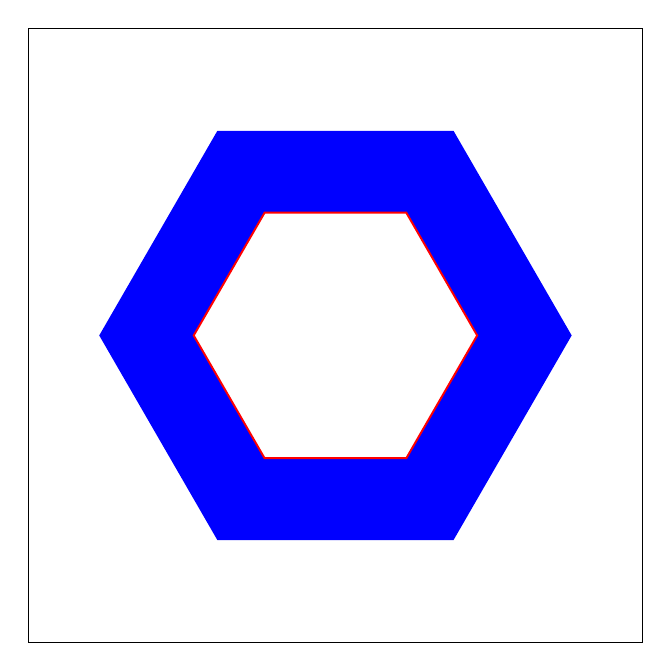
\begin{tikzpicture}[scale=3]
      \draw[line width=0.5pt, black] (-1.3,-1.3) rectangle (1.3,1.3);
      \path[fill=blue, draw=none, even odd rule]
        (0:1) -- (60:1) -- (120:1) -- (180:1) -- (240:1) -- (300:1) -- cycle
        (300:0.6) -- (240:0.6) -- (180:0.6) -- (120:0.6) -- (60:0.6) -- (0:0.6) -- cycle;
      \draw[red, line width=0.7pt]
        (0:0.6) -- (60:0.6) -- (120:0.6) --
        (180:0.6) -- (240:0.6) -- (300:0.6) -- cycle;

    \end{tikzpicture}
    \caption{Task 1: Hexagon drawing}
  \end{figure}
\end{frame}

\begin{frame}
  \begin{figure}
    \center
  \begin{tikzpicture}[scale=3]
